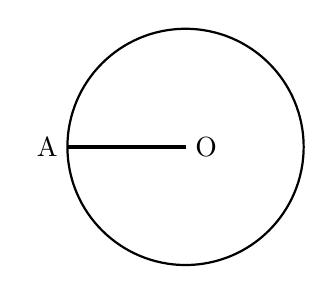
\begin{tikzpicture}[scale=1]

  % Define the center of the circle
  \coordinate (O) at (0,0);

  % Define the radius of the circle
  \def\R{1.5}

  % Draw the circle
  \draw[thick] (O) circle (\R);

  % Define point A on the left side of the circle
  \coordinate (A) at (180:\R);

  % Draw the radius line segment from center O to point A
  % Using ultra thick to match the visual weight in the image
  \draw[ultra thick] (O) -- (A);

  % Add label 'A' to the left of point A
  \node[left] at (A) {A};
  
  % Add label 'O' to the right of the center point
  \node[right] at (O) {O};

\end{tikzpicture}